\documentclass[11pt, a4paper]{article}

\usepackage[czech]{babel}
\usepackage[utf8]{inputenc}
\usepackage[T1]{fontenc}
\usepackage[left=2cm, top=3cm, text={17cm, 24cm}]{geometry}
\usepackage{times}
\usepackage{graphicx}

\begin{document}
	\begin{titlepage}
		\begin{center}
			
\includegraphics[width=0.77 \linewidth]{FIT_logo.pdf} \\

			\vspace{\stretch{0.382}}

			\Huge{Projekt 1.~část} \\
			\Huge{Datový model (ERD), model případů užití} \\
			\LARGE{\textbf{Zadání č.~2.\,--\,Marketingová (reklamní) firma [IUS]}} \\
			\Large{Databázové systémy}

			\vspace{\stretch{0.618}}
		\end{center}

		{\Large
			\today
			\hfill
			\begin{tabular}{l l}
				Jakub Komárek & (xkomar33) \\
				Lacko Dávid & (xlacko09) \\
			\end{tabular}
		}
	\end{titlepage}
	
	
	\section{Zadání}
	\qquad Vytvořte jednoduchý IS pro malou marketingovou firmu, která řeší různé zakázky. Firma je členěna na několik oddělení. U každého oddělení je třeba uchovávat jeho název, stručný popis, místnost, zaměstnance a vedoucího. Zaměstnanci pracují na jednom oddělení, je u nich uchována informace o jejich mzdě, titulu, specializaci, atp. Předpokládejte že vedoucí má na starost pouze jedno oddělení. Zakázka sestává z jednoho či více požadavků, přičemž u každého požadavku je evidován jeho typ (např. letáková kampaň, reklama v médiích, billboard, ...), cena, doba platnosti marketingové akce, počet potřebných brigádníků (ty v systému nemusíte modelovat). Požadavek může zpracovávat i více oddělení. U každé zakázky eviduje informační systém zadavatele (klienta) s jeho základními informacemi. Dále je o zakázce evidováno datum zadání, celková cena (součet cen jednotlivých požadavků), termín dodání. Každá zakázka má zodpovědného zaměstnance, který vystavuje faktury na požadavky k zakázce. Jedna faktura může být i na více požadavků. Evidujte zároveň i stav zakázky a jednotlivých požadavků (návrh, příprava, řešení, konec).
	\newpage
	
	
    \section{Diagram případů užití}
    \qquad Z diagramu vyplívá, že zaměstnanec nebude mít přístup k žádným úpravám databáze, jediná výjimka je vystavování faktur. Při práci může zobrazovat zakázky a požadavky, aby je poté zpracoval. Jeho vedoucí poté může práci průběžně monitorovat a podle toho editovat či jinak upravovat zakázky a požadavky. Vedoucí také může spravovat zaměstnance a nahlížet do faktur.\par
    Zákazník může vytvořit zakázku a poté dohlížet na její zpracování. Může také zobrazovat faktury pro něj učené. Kdyby se zákazník přestěhoval nebo si např. chtěl změnit email, je mu umožněna změna jeho kontaktních údajů.

	\begin{figure}[ht]
		\centering
		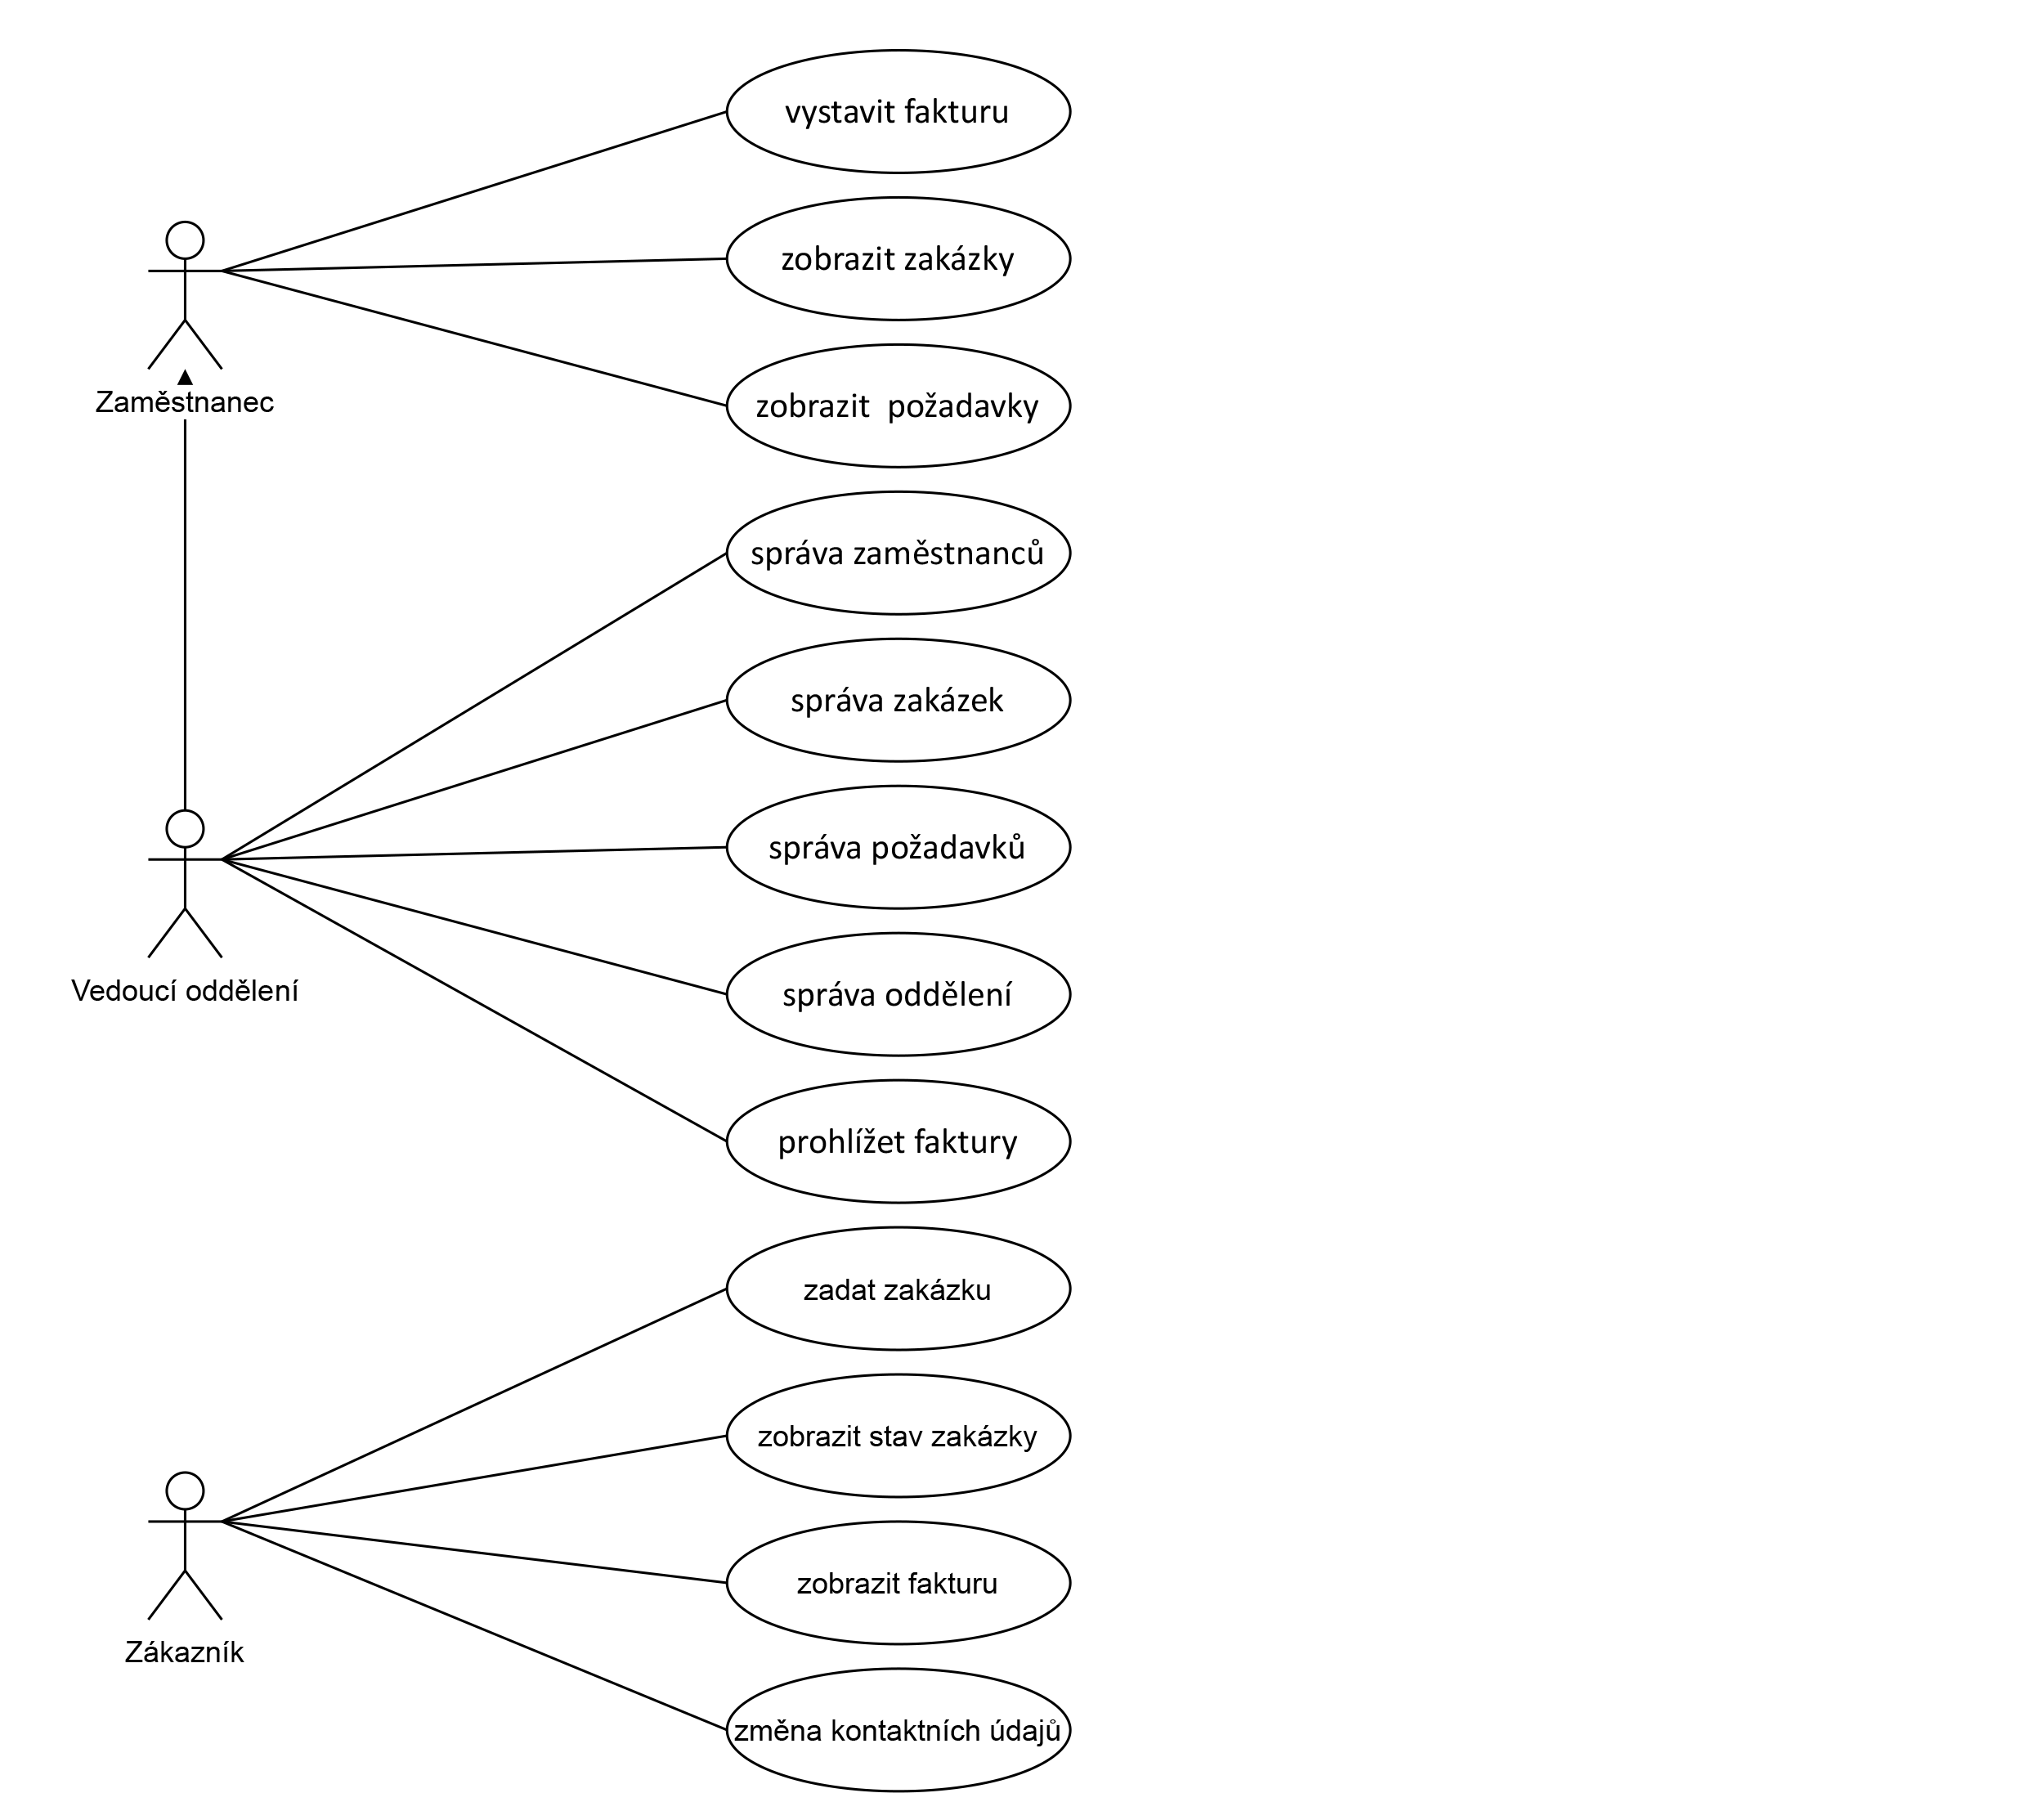
\includegraphics[width=1 \linewidth]{use_case_diagram.png}
		\caption{Model případů užití}
	\end{figure}
    \newpage
    
    
    \section{Datový model (ERD)}
    \qquad Entita osoba má jako primární klíč rodné číslo (je vždy unikátní) a uchovává se u ní základní údaje pro kontaktování osoby. Tato entita má dvě specializace klient a pracovník. U klienta není potřeba uchovávat další informace navíc. U pracovníka jsou navíc uchovány údaje o specializaci, titulu a mzdy. Pracovník musí být součástí jednoho oddělení a zároveň může být ve vztahu s oddělením jako vedoucí (může vést pouze jedno). Oddělení musí mít unikátní idedntifikátor. \par 
    Klient může být ve vztahu s 0-n objednávkami. S objednávkou je spřažen jeden odpovědný pracovník, který ji má na starost. Objednávka se skládá z jednoho či více požadavků a má svůj unikátní identifikátor. Požadavky jsou slabou entitou a pro jednoznačnou identifikaci musí být spojeny s objednávkou. Jednotlivé požadavky objednávky jsou odlišeny diskriminátorem. Faktura je spojena s pracovníkem, který ji vytvořil. Její P.K. je číslo faktury (musí se vygenerovat unikátní číslo). Faktura je přiřazena jednomu klientovy a je propojena s jedním či více požadavků.\\\\

	\begin{figure}[ht]
		\centering

		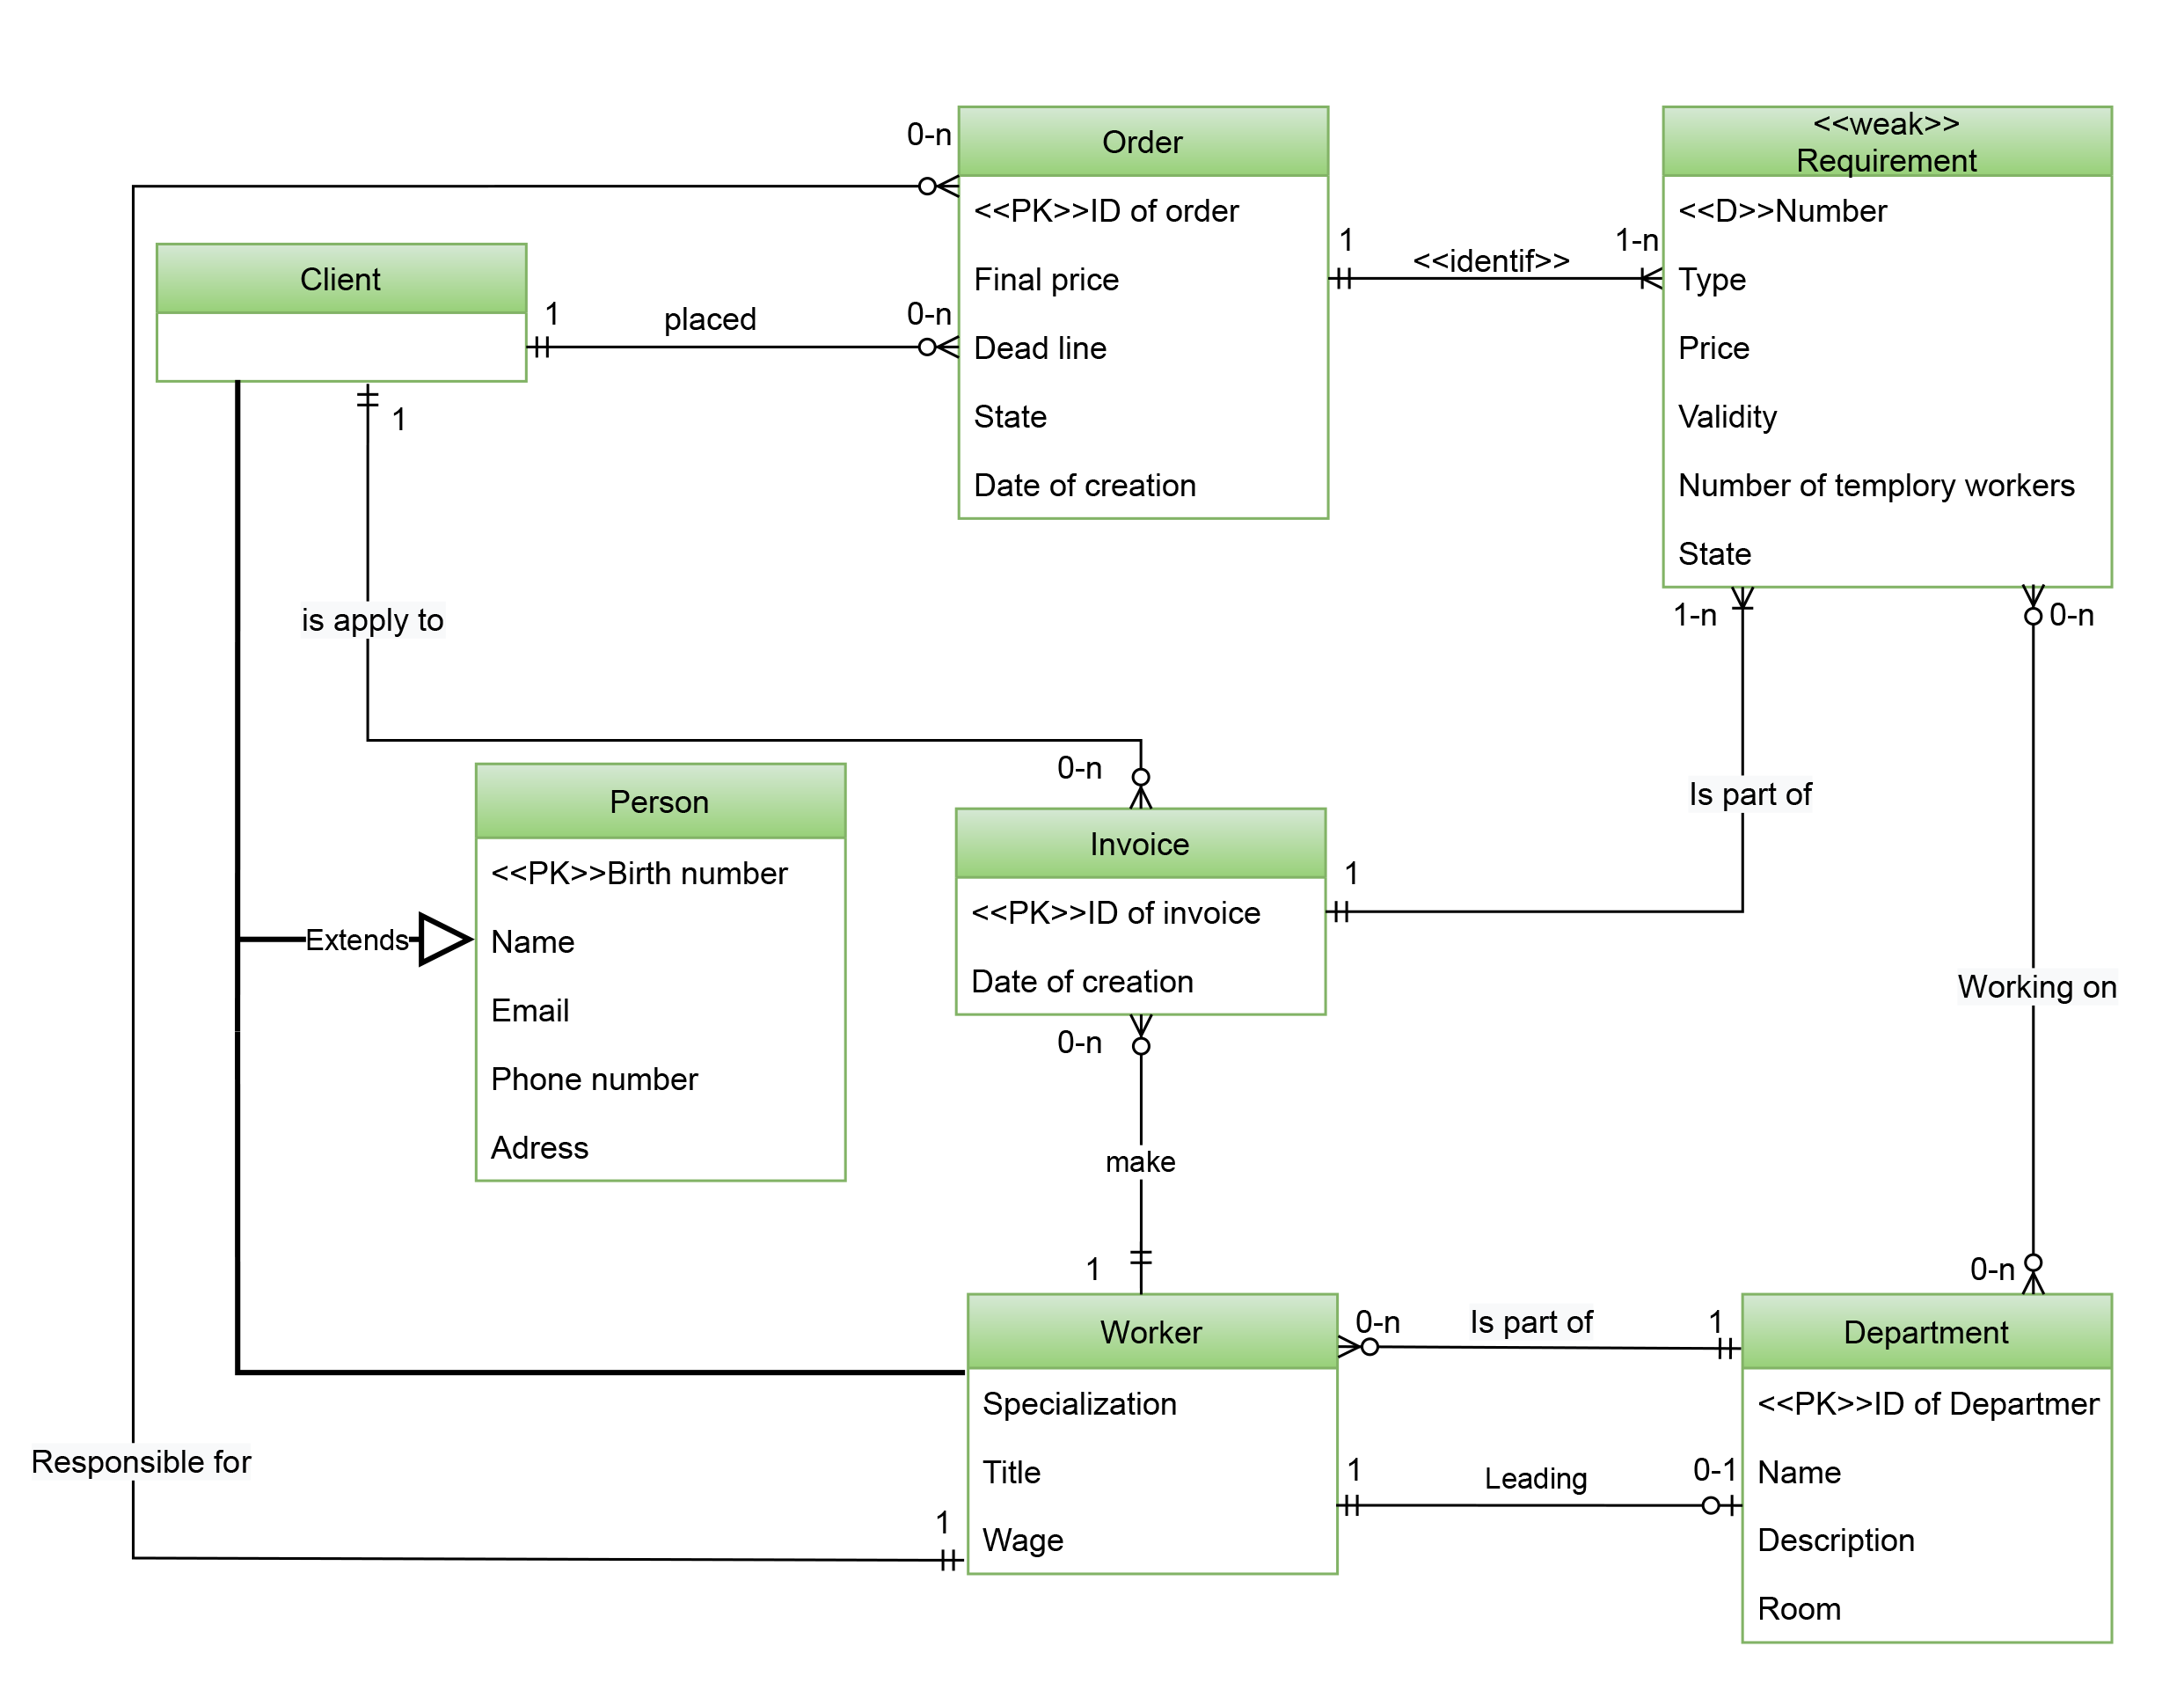
\includegraphics[width=1 \linewidth]{er_diagram.png}
		\caption{Datový model (ERD)}
	\end{figure}
\end{document}